
\section{Anomalies in neutrino oscillation observations}

\subsection{Liquid Scintillator Neutrino Detector}

The \gls{lsnd} run from 1993 to 1998 to study neutrino oscillations at the Los Alamos Meson Physics Facility.
The used Cherenkov detector contained 167t of mineral oil and was placed at only 30m distance from the target.
Interactions of neutrinos with protons, electrons and atom nuclei were observed the from 20 to 200 MeV $\bar{\nu}_\mu$-beam.

To see oscillations $\bar{\nu}_\mu \to \bar{\nu}_e$, the \gls{lsnd}-collaboration looked for electron antineutrino reactions.
Due to the proximity of the detector to the target, the expected contribution of electron neutrinos was small.
The observed rate was significatly higher than the expected value, such that it could not be explained with the common oscillation theory -- see figure \ref{fig:anomaly_plots} for an illustration.

\begin{figure*}
  \makebox[\textwidth]{%
  \begin{tikzpicture}
    % Map
    \node (img) {%
      \centering
      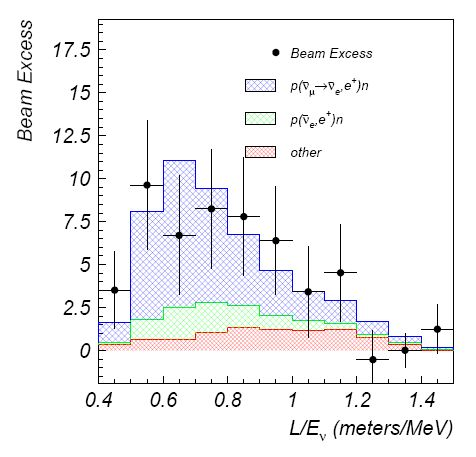
\includegraphics[width=.425\textwidth]{LSND_electrons_LoverE_dist}
      \hspace*{.5em}
      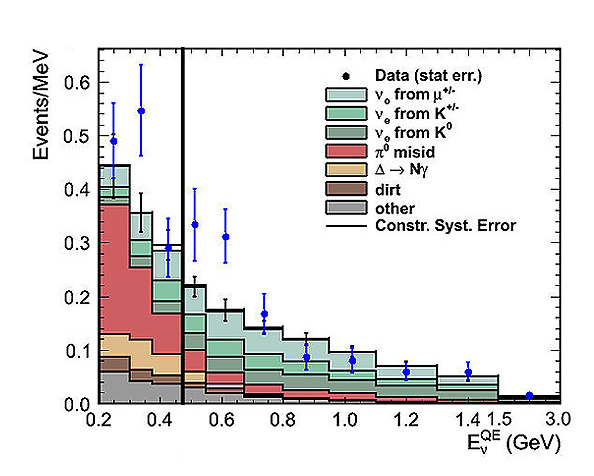
\includegraphics[width=.545\textwidth]{miniboone_excess_2}
    };
    \draw (-7.1,3.2) node[anchor=west, inner sep=1em, black] {\gls{lsnd}};
    \draw (.3,3.2)  node[anchor=west, inner sep=1em, black] {MiniBooNE};
  \end{tikzpicture}
  }
  \caption{%
    The plot on the left shows the beam excess observed by \gls{lsnd}.
    The blue region represents the required oscillation from $\bar{\nu}_\mu \to \bar{\nu}_e$.
    The plot on the right displays the excess of events at low energies observed by MiniBooNE.
  }
  \label{fig:anomaly_plots}
\end{figure*}

\subsection{MiniBooNE}

MiniBooNE was designed to observe neutrino oscillations and unambiguously verify or refute the \gls{lsnd} controversial result in a controlled environment.
The MiniBooNE detector was a Cherenkov detector located 541 m away from the target and was based on mineral-oil.\cite{Katori:2014qta}
The detector contained 800t of ultrarefined mineral oil and methylene compounds as scintillating liquid.
The experiment collected data for ten years from 2002 to 2012.

The results -- see figure \ref{fig:anomaly_plots} -- show an anomaly in the low energy distribution of the quasi-elastic neutrino events.
The observation indicate an excess of low energy electron-like events in \gls{ccqe}.\cite{Gninenko:2009ks}

